\documentclass[11pt]{article}

\usepackage{amsmath,amssymb,amsthm,setspace,tabto,fancyhdr,sectsty,mathtools}
\usepackage{titleps}
\usepackage[left=1.00in,right=1.00in,top=0.75in,bottom=1.50in]{geometry}
\usepackage{graphicx}
\graphicspath{ {assets/note3/} }

% start pdfinlimg (GPLv3, https://github.com/zerotoc/pdfinlimg/blob/master/pdfinlimg.sty)
\newcommand{\pdfinlimg}[5]{
\makebox[#1cm][l]{\immediate\pdfliteral{
  q
  #3 0 0 #4 0 0 cm
  #1 0 0 #2 0 0 cm
  0.885 0 0 0.885 0 0 cm 
  BI
  /W #3
  /H #4
  /CS /RGB
  /BPC 8
  /F [ /AHx /Fl ]
  ID
  #5>
  EI
  Q
}\vbox to #2cm{}}
}
% end pdfinlimg

% BEGIN PARAGRAPH STUFF
\usepackage[utf8]{inputenc}
\usepackage[english]{babel}
 
\setlength{\parindent}{4em}
% \setlength{\parskip}{1em}
\renewcommand{\baselinestretch}{1}
% END PARAGRAPH STUFF

% useful commands
\DeclarePairedDelimiter{\ceil}{\lceil}{\rceil}
\DeclarePairedDelimiter{\floor}{\lfloor}{\rfloor}

\newpagestyle{footers} {
    \sethead{}{}{}
    \setfoot{\small Intro to Crypto and Blockchain, Note \notenum}{\thepage}{\small Lin, Akhtar}
    \footskip = 45pt
}

\fancypagestyle{firstpage} {
    \vspace*{3\baselineskip}
    \footskip = 0pt
    \renewcommand{\headrulewidth}{6pt}
    \chead{\rule{\textwidth}{6pt} \vspace{20pt}\\}
    \lhead{\setstretch{1.05}\Large\fontfamily{lmdh}\selectfont
    Introduction to Cryptocurrencies and Blockchain 
    \\ Lin, Akhtar}
    \rhead{\huge \fontfamily{lmdh}\selectfont    Note \notenum}
    \lfoot{\small Intro to Crypto and Blockchain, Note \notenum}
    \rfoot{\small Lin, Akhtar}
}
    
\sectionfont{\Large\fontfamily{lmdh}\selectfont}

% for initial paragraph indent
\usepackage{indentfirst}

% UPDATE THIS FOR EVERY NEW NOTE
\newcommand{\notenum}{3}

\pagestyle{footers}

\begin{document}
    \thispagestyle{firstpage}
    \vspace*{2\baselineskip}
    \section*{Wallets and Cryptography}
    
    For the average user, before conducting any serious transactions, often the first step is to download wallet software to help manage funds. This note is dedicated to explaining the various types of bitcoin wallets, as well as the underlying cryptography that keeps everyone safe.
    
    \section*{Bitcoin vs Gmail Address Creation}
    
    As a brief review of the public and private keys in Bitcoin, we can compare them with that of Gmail. When generating a public/private key pair to use in Bitcoin, the user first randomly generates a private key, which is then used to calculate a public key. The set of possible private keys is so large that it is cryptographically safe to just generate a key. In contrast, the average user registering for an email account with Gmail would choose an address (username) and a password. Username and password are independent of each other in this case, and are not generated from each other, as in Bitcoin. The user would then send a request to the web server hosting , and submit this request to a central registry or mail server to check if the address is available. The main difference in the generation of public and private keys in both examples is centralization. In Bitcoin, users trust the underlying security of cryptography and the negligible probability of colliding public keys. Meanwhile, users of Gmail trust Google to safely store their private information on their servers. 
    
    \section*{Base 58}
    
    Bitcoin adopts the \textbf{base 58} convention to improve the readability of addresses. Normally, there are 26 upper case letters, 26 lower case letters, and 10 digits, totaling to 62 unique characters. To avoid confusion between visually similar characters, we drop the following characters: upper case 'I', upper case "O", lower case "l", and the digit "0". This reduces the number of possible characters to 24 upper case letters, 25 lower case letters, and 9 digits, totaling to 58 unique characters. While the majority of transactions are aided by wallet software, mitigating the possibility of misidentifying a character, reading and manually typing out one's public key is still a common enough occurrence to warrant the usage of base 58.
    
    \section*{Bitcoin Wallets}
    
    A \textbf{Bitcoin wallet} is a tool that stores a user's private key. As we will see later in this section, while wallets usually allow a user to send and receive bitcoin, as well as store a list of transactions that involve the user, there are some offline wallets that do not include this functionality. 
    
    Bitcoin wallets come in two main flavors -- hot and cold -- which describe a given wallet's connectivity to the Internet. \textbf{Hot wallets} are online and connected to the Internet. Examples of hot wallets include smartphone and PC apps such as Mycelium and AirBitz, as well as online web-wallets such as Blockchain.info and Coinbase. Smartphone and PC wallets work by storing the user's private key locally. Online services such as Coinbase store the user's private key in the cloud, thereby allowing the user to access their wallet from potentially any device. While hot wallets may excel in user experience, they are open to the many security threats of being on the Internet. A computer virus could infect a user's computer and steal the private key from a wallet PC application. Similarly, having users' private keys in the cloud requires a trusted third party to manage the users' private information.
    
    Whereas hot wallets are digital and exist on the Internet, \textbf{cold wallets} only exist in the physical world and are never connected to the Internet. Examples of cold wallets are paper wallets, hardware wallets, and brain wallets. Bitaddress.org is a popular website that uses the user's pseudo-random mouse movements to generate a private key, a public key, and a pair of QR codes. The user would then either print out the generated data or write it down manually, creating a paper wallet. Hardware wallets are external devices that sign transactions using a \textbf{trusted execution environment}. When conducting a transaction, the use would plug the hardware wallet into a PC (usually by USB) to accept unsigned transactions. The hardware wallet remains offline, signs the unsigned transaction upon, and sends the signed transaction back to the PC to broadcast to the network. Finally, brain wallets rely on the user memorizing their own private key. A common way of memorizing one's private key is to instead memorize a series of unrelated English words that hash to the private key. 
    
    \section*{Key Stretching}
    
    In regards to the aforementioned brain wallets, it is important to recognize the characteristic lack of randomness of the human mind. Specifically, a user can choose 'random' English words, but these words will inherently not be as random as those generated by computer. We also lose some randomness by only considering English words, and not random characters within the base 58 character-set. Therefore, brute-forcing another user's brain wallet could be a potential threat.
    
    To protect oneself from a brute force attack, a user could employ a process called \textbf{key stretching}. Instead of just hashing a sequence of English words, one could continue hashing the hash many times. For example, if Alice picks a sequence of English words and hashes it $2^{20}$ times, her private key would be exponentially harder to brute force. Whereas it would take her constant work to regenerate her private key, a malicious user Bob would have to first guess a sequence of English words and then guess how many times Alice's key was stretched. 
    
    \section*{Choosing a Wallet -- Multisignature Addresses}
    
    In common use, it may be useful to give control over a wallet to multiple people. However, using regular Bitcoin addresses means that any single person can steal funds from the shared wallet. \textbf{Multisignature addresses} solve this issue by requiring multiple signatures (M of N total signatures) to sign a transaction. This allows for greater security in jointly owned Bitcoin wallets. 
    
   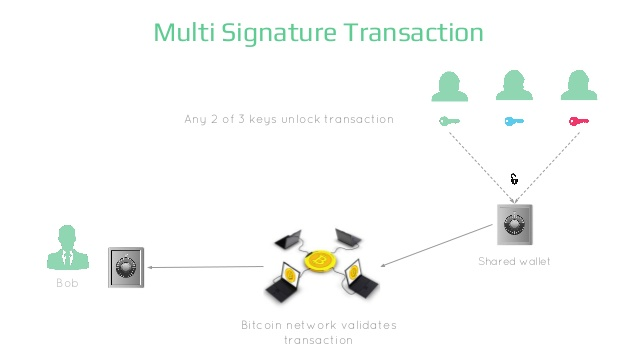
\includegraphics[scale=0.6]{multisig}

    In the image above, two of three keys in the shared wallet are necessary in order to sign a transaction. The Bitcoin network validates the transaction by checking the signature.
    
    \section*{Choosing a Wallet -- Generating New Keys}
    
    It is common practice for a user to generate new keys for every transaction. This is done for the sake of privacy. Since it is very easy for anyone to identify the public keys associated with any given transaction (on a Bitcoin block explorer for example) generating new keys for every transaction makes it hard for others to determine how much bitcoin you own, and what kinds of transactions you are taking part in. Wallet software make the process of generating and keeping track of different keys user friendly. They will do the legwork of combining funds from different keys so that the user can see exactly how much bitcoin they have, while enjoying reinforced security. 
    
    \section*{Choosing a Wallet -- Wallet Backups}
    
    Wallet backups are imperative to protect against potential hardware failures, where the loss of a wallet could potentially mean losing all of one's bitcoin. However, generating new keys for every transaction poses a problem in terms of wallet backups. If a user generates a new address every time they want to conduct a transaction, then the safest backup scheme would be to create a new backup for every new address. This backup scheme is characteristic of \textbf{JBOK (Just a Bunch of Keys) wallets}.
    
    Clearly, there was a better way to handle wallet backups, so in \textbf{BIP (Bitcoin Improvement Proposal)} 32, the Bitcoin protocol expanded to allow for \textbf{HD (hierarchical deterministic) wallets}. This determined a proccess whereby a 'child' private key could be derived from a 'parent' private key using secure mathematical relationships. The mathematical properties of deterministic systems ensures that child private keys can always be calculated from parent private keys, decreasing the need to back up all keys upon every transaction, as we saw with JBOK wallets. Additionally, each parent private key can have multiple child private keys, and each child private key can in turn be a parent private key and have children as well, defining the hierarchical property of HD wallets.  

   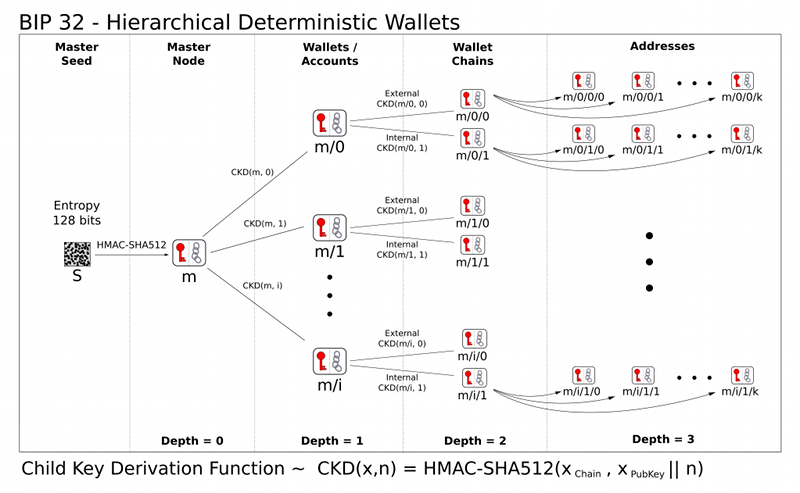
\includegraphics[scale=4]{bip32}
   
   Usage of HD wallets, especially when used in such schemes as the one shown above, is useful in the context of complex organizations. A potential set up could be as follows: A master seed would be generated and kept secret. Financial officers or the CEO would then control the master node (private key). Wallets/accounts would then be distributed to every department of the organization, and the department would then distribute wallets to each of their employees, creating a useful and very manageable hierarchical structure.
   
   \section*{Choosing a Wallet -- Control \& Responsibility}
   
   Now we will explore some of the most noteworthy wallets, and explain how each of them differ in terms of the user's level of control and responsibility over their own funds.
   
   We previously mentioned that services such as Coinbase store users' private keys in the cloud. This allows Coinbase to potentially spend or move your funds, as long as your balance stays the same whenever you use your wallet. In this sense, Coinbase functions like a centralized bank (which some Bitcoin enthusiasts do not appreciate.) The advantage to having a centralized organization holding your private keys is that in the case you forget your Coinbase password, all it takes is an email or phone call for you to retrieve your funds.
   
   On the other hand, services such as Mycelium and Electrum do not hold anyone's private keys. They make it clear that users themselves hold their own private keys, and that they are responsible for their own funds. There is no recourse in the case of a forgotten key or lost funds. The benefit of course is the security of knowing that no one else controls your private keys. However, the lack of a safety net in the case of the loss of a key may scare users away.
   
   As somewhat of a compromise, hardware wallets such as Case Wallet require 2 of 3 signatures (or any other multi-signature scheme) to sign a transaction. Three signatures are delegated to the the device, Case service, and a separate backup company. When a user wants to conduct a transaction, the two necessary signatures are provided by their device as well as the Case service. In the case of a lost device, a user can call Case and the separate backup company, a necessary 2 of 3 signatures, to retrieve funds.
   
   
   %some sort of transition here? 
   
   \section*{Cryptographic Hash Functions}
   
   A \textbf{cryptographic hash function} is a function that maps some \underline{arbitrarily-sized it string} to some \underline{fixed-size bit string}. 
   
   $$H:~ \{0,1\}^{*} \mapsto \{0,1\}^{k}$$
   
   SHA-256 is an example of a cryptographic hash function that is used extensively in the Bitcoin protocol. A cryptographic hash function only \underline{evaluates in one direction}, meaning that it is difficult to find an input given just the output it generates. Cryptographic hash functions are also \underline{deterministic}, meaning that there is no sense of randomness in the system, and that the same input always yields the same output. 
   
   The \textbf{avalanche effect} of cryptographic hash functions describes how a slight change in a function's input drastically changes its corresponding output. The avalance effect is important because we want the hash values to be close to uniformly random over the entire output space.
   
   \textbf{Preimage resistance} is also a desired characteristic of good cryptographic hash functions, and describes that it should be extremelly difficult to find the preimage of a cryptographic hash function output. Formally,
   
   \begin{align*}
       x &= \{0,1\}^{*} = \text{message (preimage)} \\
       y &= H(x) = \text{hash (output)} \\
       x &= H^{-1}(y) \rightarrow \text{finding the message should be computationally difficult}
   \end{align*}
   
   \textbf{Second preimage resistance} tells us that in a good cryptographic hash function, it should be extremely difficult to find any value that maps to a specific input. Formally, for any given message $x$, finding any $x'$ such that $H(x') = H(x)$ should be computationally difficult.
   
   Finally, \textbf{collision resistance} in hash functions tells us that the probability of finding two inputs that map to the same output is very small. There are two equivalent ways of formalizing this statement. Suppose we have two messages $x_1$ and $x_2$;
   
   \begin{enumerate}
       \item The probability that their hashes are equal, $P\big(H(x_1) = H(x_2)\big)$, is very small, or
       \item finding \textit{any} $x_1,~x_2$ such that $H(x_1)=H(x_2)$ is computationally difficult.
   \end{enumerate}
   
   \section*{Use of Cryptographic Hash Functions}
   
   In the context of Bitcoin, we have seen cryptographic hash functions used in a number of places. You can use SHA-256 to prove the existence of certain data points inside of a merkle tree, and this is what miners do when they verify transactions. Evaluation of SHA-256 is used as proof-of-work. Also, transactions, blocks, and addresses are all referenced by hash value. Outside of Bitcoin and cryptocurrencies, cryptographic hash functions find use in applications such as: hash-based message authentication codes (HMACs), password verification, commitment schemes, pseudo-random number generators (PRNGs), and as being the fundamental operation in most cryptographic protocols. 
   
    \section*{Simple Hash Commitment Scheme}
   
    In this section, we will display the useful properties of cryptographic hash functions in a simple example. Consider a scenario where Alice and Bob each bet \$100 on a coin flip. Alice calls the outcome of the coin flip, and BBob bflips the coin. If Alice guesses correctly the outcome of the coin flip, she wins \$200. This scenario is simple enough to execute, with little room for error. However, what if Alice and Bob are \underline{separated} and \underline{do not trust one another}? Since Alice and Bob are separated, it is very easy for Bob to cheat. Alice would send Bob a message containing her guess, and Bob would simply send back a message saying the outcome was the opposite of what Alice guessed (so Bob gets to keep his money.)
    
    The solution to this problem can be solved by binding Alice's guess with a \textbf{commitment}:
    
    \begin{enumerate}
        \item Alice first chooses a large random number, $R$
        \item Alice guesses the outcome of the coin flip, $B$
        \item Alice generates a commitment to the coin flip by concatenating her guess with the random number, and hashing the result: $C = H(B||R)$
        \item Alice sends this commitment to Bob
        \item Bob flips the coin and sends the result back to Alice
        \item Alice sends Bob the random number and her guess: $(R', B')$
        \item Bob then checks that $C' = H(R'||B')==C=H(B||R)$, to ensure that Alice did not changer her guess mid-commitment
        \item Both Alice and Bob can now agree on who won the \$200
    \end{enumerate}
    
    The scheme developed above depends on the effectiveness of our function $H$, and whether or not it has the essential properties of a good cryptographic hash function. Some exampes easily illustrate the necessity for these properties.
    
    When Bob receives the commitment $C=H(B||R)$ from Alice, if he can compute $H^{-1}(C) = B||R$, Bob can recover Alice's guess and send her the opposite outcome. However, if our hash function $H$ is \underline{preimage resistant}, this should not be possible, as finding the input for a given output is computationally difficult.
    
    Another way to potentially break the system would be if Alice sends Bob her commitment $C=H(B||R)$ as before, but reveals the opposite guess $(B!,R')$ instead. Alice wins the bet if she can pick $R'$ such that $C'=H(!B||R') = C$ However, if our hash function $H$ is \underline{second preimage resistant}, this scenario is impossible
    
    
    

    % BEGIN KEY TERMS
    \newpage
    \thispagestyle{firstpage}
    \vspace*{2\baselineskip}
    \section*{Key Terms}
    \noindent A collection of terms mentioned in the note which may or may not have been described. Look to external sources for deeper understanding of any non-crypto/blockchain terms.
    \begin{enumerate}
        % edit within here
        \item \textbf{VOCAB WORD} --- Definition. % format
    \end{enumerate}
    % END KEY TERMS
\end{document}